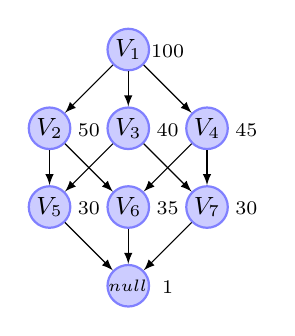
\begin{tikzpicture}[main_node/.style={circle,fill=blue!20,draw=blue!50,thick,
	minimum size=1.5em,inner sep=0pt,font=\small},
edge from parent/.style={->,draw},>=latex]
  
    \node[main_node,label={[shift={(0.5,-0.5)}]{\scriptsize 40}}] (1) at (0, 0) {$V_3$};
    \node[main_node,label={[shift={(0.5,-0.5)}]{\scriptsize 45}}] (2) at (1, 0)  {$V_4$};
    \node[main_node,label={[shift={(0.5,-0.5)}]{\scriptsize 50}}] (3) at (-1, 0) {$V_2$};
	\node[main_node,label={[shift={(0.5,-0.5)}]{\scriptsize 35}}] (4) at (0, -1) {$V_6$};
	\node[main_node,label={[shift={(0.5,-0.5)}]{\scriptsize 30}}] (5) at (1, -1) {$V_7$};
	\node[main_node,label={[shift={(0.5,-0.5)}]{\scriptsize 30}}] (6) at (-1, -1) {$V_5$};
	\node[main_node,label={[shift={(0.5,-0.5)}]{\scriptsize 100}}] (7) at (0, 1) {$V_1$};
	\node[main_node,label={[shift={(0.5,-0.5)}]{\scriptsize 1}}] (8) at (0, -2) {$_{null}$};

    \draw[->] (7) -- (3);
	\draw (7) edge[->] (2);
	\draw (3) edge[->] (4);
	\draw (2) edge[->] (4);
	
	\draw (1) edge[->] (6);
	\draw (1) edge[->] (5);
	\draw (6) edge[->] (8);
	\draw (5) edge[->] (8);
	
	\draw (7) edge[->] (1);
	\draw (3) edge[->] (6);
	\draw (4) edge[->] (8);
	\draw (2) edge[->] (5);
\end{tikzpicture}